% =============================================================================
% MIVA-KNIGHT — Full methodology flowchart (training + inference)
% Compile: pdflatex MIVA_KNIGHT_Methodology_Flowchart.tex
% Requires: tikz (positioning, shapes, arrows.meta, calc, fit, backgrounds)
% =============================================================================
\documentclass[11pt,a4paper,landscape]{article}
\usepackage[margin=0.6in]{geometry}
\usepackage{tikz}
\usetikzlibrary{shapes.geometric,arrows.meta,positioning,calc,fit,backgrounds,matrix}

\usepackage{graphicx}
\usepackage{xcolor}
\usepackage{amsmath}
\usepackage{enumitem}
\usepackage[hidelinks]{hyperref}

\definecolor{trainbg}{RGB}{230,242,255}
\definecolor{pipelinesbg}{RGB}{220,245,230}
\definecolor{kgbg}{RGB}{255,245,220}
\definecolor{inferblue}{RGB}{210,225,250}
\definecolor{infergreen}{RGB}{210,240,220}
\definecolor{inferguard}{RGB}{255,228,228}
\definecolor{infergen}{RGB}{232,218,245}

\tikzset{
  arr/.style={-{Stealth[length=2.4mm]}, thick, draw=black!55},
  darr/.style={-{Stealth[length=2.4mm]}, thick, dashed, draw=black!45},
  lbl/.style={font=\scriptsize\sffamily\bfseries},
  small/.style={font=\tiny\sffamily},
  box/.style={rectangle, rounded corners=3pt, draw=black!55, align=center, inner sep=4pt, minimum width=2.1cm},
  phase/.style={rectangle, rounded corners=4pt, inner sep=8pt, thick}
}

\begin{document}
\thispagestyle{empty}
\begin{center}
{\Large\sffamily\bfseries MIVA-KNIGHT --- Full Methodology Flowchart}\\[4pt]
{\small\sffamily Training pipelines (offline) + hybrid RAG inference (runtime), aligned with
\texttt{MIVA\_KNIGHT\_Complete\_Thesis\_Final.tex} and implementation notebooks.}
\end{center}
\vspace{0.35cm}

% --- SCALE: whole diagram fits landscape A4 ---
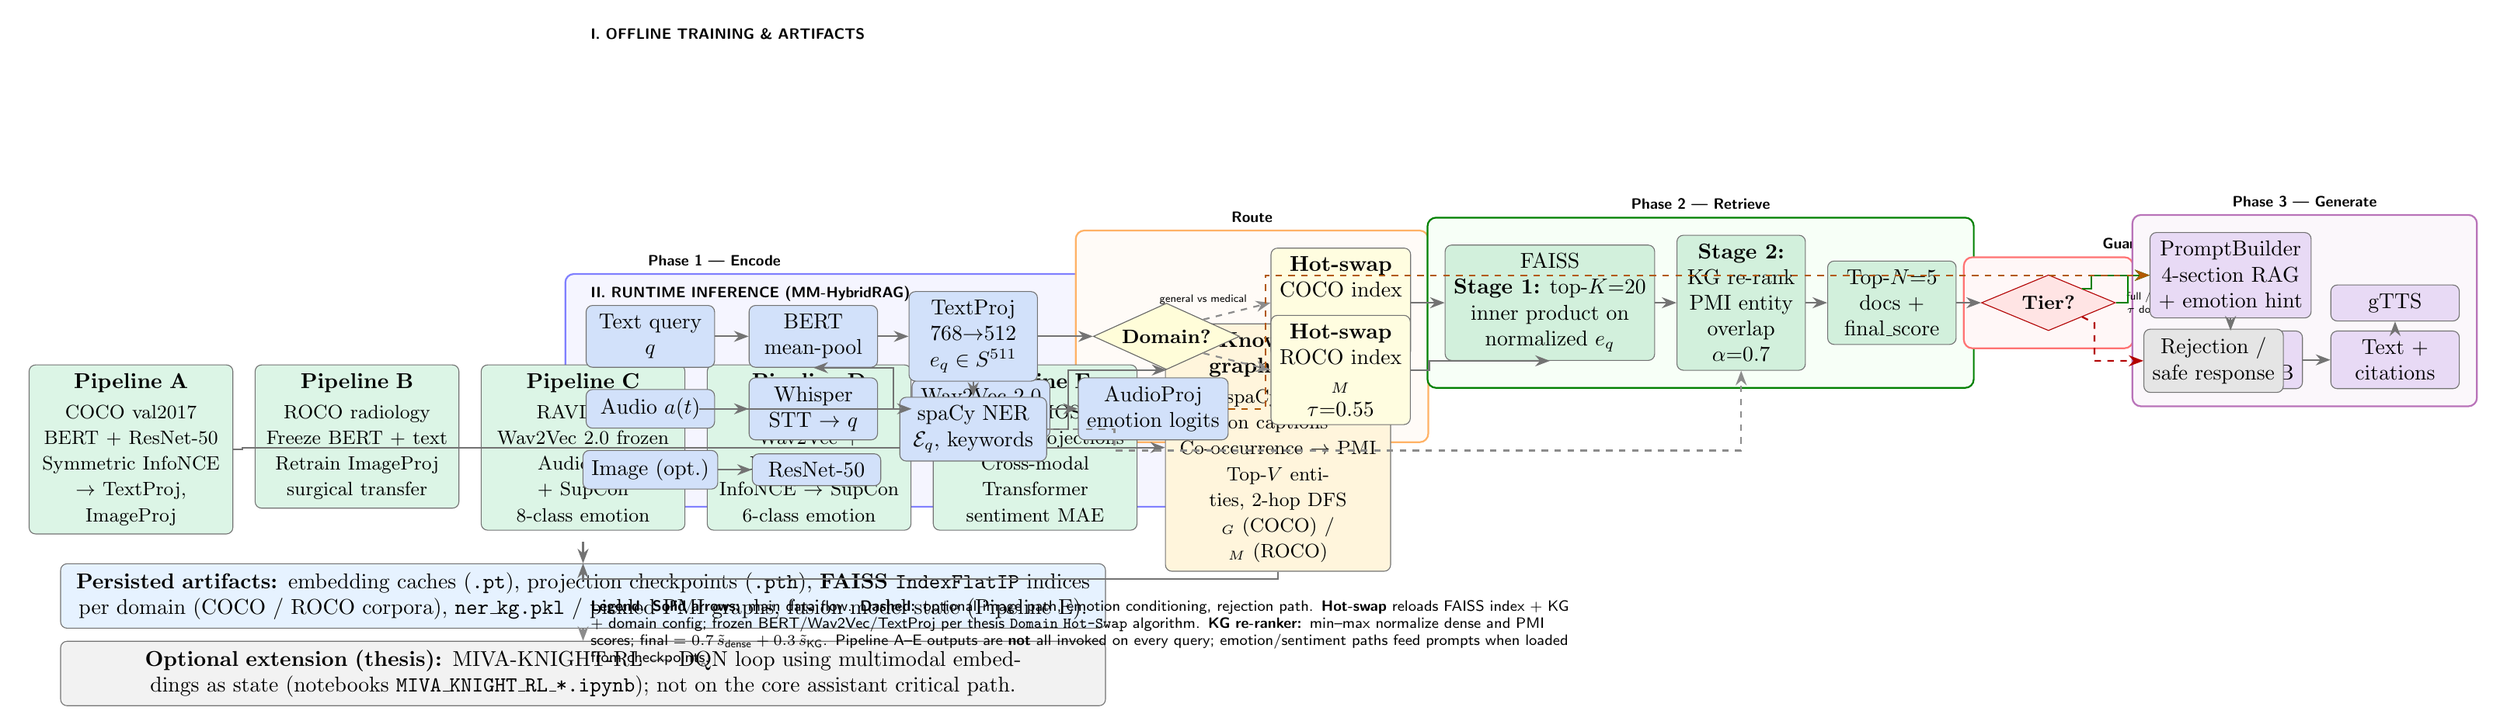
\begin{tikzpicture}[node distance=0.22cm and 0.28cm, transform shape]

  % =========================  PART I: OFFLINE TRAINING  =========================
  \node[lbl, anchor=west] (titletrain) at (0,6.8) {I. OFFLINE TRAINING \& ARTIFACTS};

  % Row: five pipelines
  \matrix (pipelines) [matrix of nodes, column sep=0.35cm, row sep=0.12cm,
    nodes={box, fill=pipelinesbg, minimum height=1.35cm, text width=3.05cm}]
  {
    {\textbf{Pipeline A}\\[2pt]{\small COCO val2017}\\{\small BERT + ResNet-50}\\{\small Symmetric InfoNCE}\\{\small $\rightarrow$ TextProj, ImageProj}} &
    {\textbf{Pipeline B}\\[2pt]{\small ROCO radiology}\\{\small Freeze BERT + text}\\{\small Retrain ImageProj}\\{\small surgical transfer}} &
    {\textbf{Pipeline C}\\[2pt]{\small RAVDESS}\\{\small Wav2Vec 2.0 frozen}\\{\small AudioProj + SupCon}\\{\small 8-class emotion}} &
    {\textbf{Pipeline D}\\[2pt]{\small CREMA-D}\\{\small Wav2Vec + ResNet frame}\\{\small InfoNCE $\rightarrow$ SupCon}\\{\small 6-class emotion}} &
    {\textbf{Pipeline E}\\[2pt]{\small CMU-MOSI}\\{\small Frozen 3 projections}\\{\small Cross-modal Transformer}\\{\small sentiment MAE}} \\
  };

  % KG construction box
  \node[box, fill=kgbg, text width=3.4cm, minimum height=1.35cm, right=0.45cm of pipelines-1-5.east, anchor=west] (kgbuild)
    {\textbf{Knowledge graph (PMI)}\\[2pt]{\small spaCy NER on captions}\\{\small Co-occurrence $\rightarrow$ PMI}\\{\small Top-$V$ entities, 2-hop DFS}\\{\small $\KG_G$ (COCO) / $\KG_M$ (ROCO)}};

  \draw[arr] (pipelines-1-1.east) -- ++(0.15,0) |- (kgbuild.west);

  % Artifacts strip
  \node[box, fill=trainbg, text width=16.8cm, minimum height=0.95cm, below=0.35cm of pipelines.south, anchor=north] (artifacts)
    {\textbf{Persisted artifacts:} embedding caches (\texttt{.pt}), projection checkpoints (\texttt{.pth}),
    \textbf{FAISS} \texttt{IndexFlatIP} indices per domain (COCO / ROCO corpora),
    \texttt{ner\_kg.pkl} / pickled PMI graphs, fusion model state (Pipeline E).};

  \node[box, fill=gray!10, text width=16.8cm, minimum height=0.55cm, below=0.2cm of artifacts] (rlopt)
    {\textbf{Optional extension (thesis):} MIVA-KNIGHT-RL --- DQN loop using multimodal embeddings as state (notebooks \texttt{MIVA\_KNIGHT\_RL\_*.ipynb}); not on the core assistant critical path.};

  \draw[arr] (pipelines.south) -- ++(0,-0.12) -| (artifacts.north);
  \draw[arr] (kgbuild.south) -- ++(0,-0.12) -| (artifacts.north);
  \draw[darr] (artifacts.south) -- (rlopt.north);

  % =========================  PART II: RUNTIME INFERENCE  =========================
  \node[lbl, anchor=west] (titleinf) at (0,2.55) {II. RUNTIME INFERENCE (MM-HybridRAG)};

  % Inputs
  \node[box, fill=inferblue] (inq) at (1.1,1.85) {Text query\\$q$};
  \node[box, fill=inferblue, below=0.35cm of inq] (ina) {Audio $a(t)$};
  \node[box, fill=inferblue, below=0.35cm of ina] (ini) {Image (opt.)};

  % Encoding lane
  \node[box, fill=inferblue, right=0.55cm of inq] (bert) {BERT\\mean-pool};
  \node[box, fill=inferblue, right=0.55cm of ina] (whisper) {Whisper\\STT $\rightarrow$ $q$};
  \node[box, fill=inferblue, right=0.55cm of ini] (resin) {ResNet-50};
  \node[box, fill=inferblue, right=0.55cm of whisper] (w2v) {Wav2Vec 2.0\\emotion};

  \node[box, fill=inferblue, right=0.5cm of bert] (tproj) {TextProj\\$768{\to}512$\\$e_q\in\mathbb{S}^{511}$};
  \node[box, fill=inferblue, below=0.25cm of tproj, minimum width=2.4cm] (ner) {spaCy NER\\$\mathcal{E}_q$, keywords};

  \node[box, fill=inferblue, right=0.45cm of w2v] (ap) {AudioProj\\emotion logits};

  \draw[arr] (inq) -- (bert);
  \draw[arr] (ina) -- (whisper);
  \draw[arr] (whisper.east) -| ++(0.25,0.6) |- (bert.south);
  \draw[arr] (ina) -- ++(0.8,0) |- (w2v.west);
  \draw[arr] (ini) -- (resin);
  \draw[arr] (bert) -- (tproj);
  \draw[arr] (tproj) -- (ner);
  \draw[arr] (w2v) -- (ap);

  % Domain router
  \node[diamond, aspect=2.2, draw=black!60, fill=yellow!15, inner sep=2pt, right=0.9cm of tproj] (dom) {\small\textbf{Domain?}};
  \node[small, above=0.12cm of dom.north east] {general vs medical};

  \draw[arr] (tproj.east) -- (dom.west);
  \draw[arr] (ner.east) -| ++(0.35,0) |- (dom.south);

  \node[box, fill=yellow!12, right=0.5cm of dom, yshift=0.55cm] (swapg) {\textbf{Hot-swap}\\COCO index\\$\KG_G$\\$\tau{=}0.40$};
  \node[box, fill=yellow!12, right=0.5cm of dom, yshift=-0.55cm] (swapm) {\textbf{Hot-swap}\\ROCO index\\$\KG_M$\\$\tau{=}0.55$};

  \draw[darr] (dom.north east) -- (swapg.west);
  \draw[darr] (dom.south east) -- (swapm.west);

  % Retrieval
  \node[box, fill=infergreen, right=0.35cm of swapg.east, anchor=west, xshift=0.2cm] (faiss) {FAISS\\\textbf{Stage 1:} top-$K{=}20$\\inner product on\\normalized $e_q$};
  \node[box, fill=infergreen, right=0.35cm of faiss] (kgrr) {\textbf{Stage 2:}\\KG re-rank\\PMI entity\\overlap\\$\alpha{=}0.7$};
  \node[box, fill=infergreen, right=0.35cm of kgrr] (top5) {Top-$N{=}5$\\docs +\\final\_score};

  \draw[arr] (swapg.east) -- (faiss.west);
  \draw[arr] (swapm.east) -- ++(0.3,0) |- (faiss.south);
  \draw[arr] (faiss) -- (kgrr);
  \draw[arr] (kgrr) -- (top5);
  \draw[darr] (ner.east) -| ++(1.1,-0.35) -| (kgrr.south);

  % Confidence
  \node[diamond, aspect=2.4, draw=red!70!black, fill=inferguard, right=0.4cm of top5] (conf) {\small\textbf{Tier?}};
  \node[small, right=0.05cm of conf.east, text width=2.1cm] {full / partial / rejected\\$\tau$ domain};

  \draw[arr] (top5) -- (conf);

  % Generation
  \node[box, fill=infergen, right=0.55cm of conf, yshift=0.45cm] (pb) {PromptBuilder\\4-section RAG\\+ emotion hint};
  \node[box, fill=infergen, below=0.2cm of pb] (llm) {Groq API\\Llama-3.1-8B};
  \node[box, fill=infergen, right=0.45cm of llm] (out) {Text +\\citations};
  \node[box, fill=infergen, above=0.15cm of out] (tts) {gTTS};

  \node[box, fill=gray!20, right=0.45cm of conf, yshift=-0.95cm] (rej) {Rejection /\\safe response};

  \draw[arr, color=green!50!black] (conf.north east) -- ++(0.15,0) |- (pb.west);
  \draw[arr, color=green!50!black] (conf.east) -- ++(0.2,0) |- (pb.west);
  \draw[arr] (pb) -- (llm);
  \draw[arr] (llm) -- (out);
  \draw[arr] (out) -- (tts);
  \draw[darr, color=orange!70!black] (ap.east) -| ++(0.6,0.5) |- (pb.west);
  \draw[arr, color=red!70!black, dashed] (conf.south east) -- ++(0.2,-0.1) |- (rej.west);

  % Background phases
  \begin{scope}[on background layer]
    \node[phase, draw=blue!50, fill=blue!4, fit=(inq)(ina)(ini)(bert)(whisper)(resin)(w2v)(tproj)(ner)(ap), label={[lbl]above left:Phase 1 --- Encode}] {};
    \node[phase, draw=orange!60, fill=orange!3, fit=(dom)(swapg)(swapm), label={[lbl]above:Route}] {};
    \node[phase, draw=green!50!black, fill=green!3, fit=(faiss)(kgrr)(top5), label={[lbl]above:Phase 2 --- Retrieve}] {};
    \node[phase, draw=red!55, fill=red!3, fit=(conf), label={[lbl]above right:Guard}] {};
    \node[phase, draw=violet!55, fill=violet!3, fit=(pb)(llm)(out)(tts), label={[lbl]above:Phase 3 --- Generate}] {};
  \end{scope}

  % Legend
  \node[anchor=north west, font=\scriptsize\sffamily, text width=16cm] at (0,-2.35) {
    \textbf{Legend.} \textbf{Solid arrows:} main data flow. \textbf{Dashed:} optional image path, emotion conditioning, rejection path.
    \textbf{Hot-swap} reloads FAISS index + KG + domain config; frozen BERT/Wav2Vec/TextProj per thesis \texttt{Domain Hot-Swap} algorithm.
    \textbf{KG re-ranker:} min--max normalize dense and PMI scores; $\text{final} = 0.7\,\tilde{s}_{\text{dense}} + 0.3\,\tilde{s}_{\text{KG}}$.
    Pipeline A--E outputs are \textbf{not} all invoked on every query; emotion/sentiment paths feed prompts when loaded from checkpoints.
  };

\end{tikzpicture}

\vfill
\begin{center}
{\scriptsize\sffamily Oluwakayode Soyinka --- MIVA-KNIGHT methodology diagram --- \today}
\end{center}

\end{document}
